\documentclass{school-22.101-notes}
\date{November 9, 2011}

\begin{document}
\maketitle


%%%%%%%%%%%%%%%%%%%%%%%%% Part 3: Radioactive Decay %%%%%%%%%%%%%%%%
\lecture{Radioactive Decay}
In this chapter, we discuss two topics: 
\begin{enumerate}
\item How do we describe mass? $M(A,Z)$. 
  \begin{enumerate}
  \item We consider binding energy vs. A, which yields the binding energy curve. 
  \item We consider for a fix $A$, M vs. Z (it's a concave up curve). 
  \end{enumerate}

\item Then we move from stable cases (nuclear binding) to the unstable cases (transition), including:
  \begin{itemize}
  \item Spontaneous decays: spontaneous transitions, this chapter. 
  \item Nuclear reactions: induced transition (bombarded with particles), very important, next chapter.   
  \end{itemize}
Example: \ce{^1H ->[+n] ^2_1H_1 ->[+n] ^3H} (stable)  \ce{->[\beta] ^3He} (unstable) \ce{ ->[+n] ^4He} (very stable, because double magic 2n + 2p). 

\ce{^4He} can get a neutron to become \ce{^5He}, but the half life is very short ($3 \times 10^{-21}$ s); similarly if \ce{^4He} gets a proton to form \ce{^5Li} its half-life is on the order of $10^{-22} \s$. It appears that it is impossible to make heavy nuclei, which is of course not the case. This leads us to the inter-connection between nuclei mass, binding energy, and energy released or absorbed in nuclear reactions.
\end{enumerate}




\topic{Fundamentals}
\begin{enumerate}
\item Know the plot of $\Delta$ vs. $A$ which is a concave up curve with a range of values in the negative range. 

\item Expressing mass in energy, $1 u = 1.66 \times 10^{-24} \g = 931.48 \MeV$. $1 e = 0.511 \MeV, 1 p = 938.3 \MeV, 1 n = 939.6 \MeV$ (half-life: 13 mins). 

\item 
\end{enumerate}

\topic{Binding Energy}
Binding energy of a nucleus with A,Z is:
\begin{align} 
B(A,Z) &= \left[ Z m_p + N m_n - (m(A,Z) - Z m_e) \right] c^2 \\
&= \left[ Z m_{\ce{^1 H}} + N m_n - m(A,Z) \right] c^2
\end{align}
Binding energy for the outmost neutron (`valence' nucleon) $=$ neutron separation energy $=$ the energy required to separate one neutron from a nucleus; similarly for proton separation energy: 
\begin{align}
S_n &= B(\ce{^A_Z X_N}) -B(\ce{^{A-1}_Z X_{N-1}}) = \left[ m(A-1, Z) - m(A,Z) + m_n \right] c^2 \\
S_p &= B(\ce{^A_Z X_N}) -B(\ce{^{A-1}_{Z-1} X_{N}}) = \left[ m(A-1, Z-1) - m(A,Z) + m_{H} \right] c^2
\end{align}

\begin{enumerate}
\item Binding Energy as a Function of A. 
\begin{enumerate}
\item As $A$ increases, Total Binding Energy increases. Binding energy is always positive. 
\item BE per nucleon, $B/A$, is not a linear relationship with $A$. \hi{Increasing $B/A$ means forming a more tightly bound product, thus releasing energy.} There are two ways to release energy: 
    \begin{enumerate}
    \item For small A up to $A = 60$ (\ce{^{56} Fe}, \ce{^{58} Fe}, \ce{^{62} Ni}), B/A, hence the isotopes become more stable; hence fusion is applicable in this region because we gain energy as we bring small A particles together; 
    \item Beyond $A = 60$, as A increases, B/A decreases very gradually, relatively constant for most nuclei with B/A around 8 MeV. Fission is applicable in this case because we can gain energy by splitting/decreasing A. 
    \end{enumerate}  
\end{enumerate}


\item Neutron separation energy is the binding energy of the last neutron: 
  \eqn{ S_n = [M_n + M(A-1, Z) - M(A,Z)] c^2 }
  FIXME: insert Fig.10.2. The difference between even and odd is about 1 MeV. This is why U238 undergoes only fast fission, whereas U235 can undergo thermal fission. At 1 MeV, $\sigma_f (U235) = 700b, \sigma_f (U238) = 1b$. 


\item Contributors of Binding Energy: Volume Effect (positive effect), Surface Effect (negative effect because less nucleon interaction on the surface), Coulomb Interaction (negative effect), Asymmetry Effect (negative effect), Parity Effect (can be positive, negative, or no effect). 
\begin{enumerate}
    \item Volume Contribution: An initial guess is that, each nucleon would interact with any other nucleon (A-1 of them); so together the volume contribution is proportional to $A(A-1) \approx A^2$. This is not quite right because nuclear interactions are short range (strong nuclear force). Assume that each nucleon has about the same number of neighbors (except on the surface -- surface effect would take into account this part), hence the volume term should be roughly proportional to $A$:
    \eqn{B_V = 15.5 \MeV A} 

    \item Surface Contribution: Surface nucleons are surrounded by less neighbors than the bulk (inner) nucleons. The surface nucleons do not contribute to B as much, hence we need to subtract from the binding energy a term proportional to the surface area, which is 2/3 power of the volume (or, say A). Experimental data tells us $a_S \approx a_V$ as expected. 
    \eqn{B_S = - 16.8 \MeV A^{2/3}}

    \item Coulomb Contribution: the coulomb repulsion of protons make nucleus less tightly bound. For a total charge is $Ze$, we consider a constant charge distribution $\rho = \frac{Ze}{\frac{4\pi}{3} R^3}.$ If we consider a small shell from $r$ to $r + \dr$, then the Coulomb force between the spherical core and the shell is 
    \eqn{ \int_0^{R} \frac{1}{r} \underbrace{\left( \frac{4}{3} \pi r^3 \rho \right)}_{\mathrm{core}} \underbrace{\left(\rho \cdot 4 \pi r^2 \dr \right)}_{\mathrm{shell}} = \frac{3}{5} \frac{Z^2 e^2}{R}.}
    Then we have to correct the term by taking into account the `self-energy' of each proton with the magnitude of $\frac{3e^2}{5R}$ (this term arises from that we assume the charges of protons `smeared' over the entire nucleus, hence under this assumption each proton would repel itself as well), so the result is ($r_0 = 1.2 \fm$):
    \eqn{V_{coul} = \frac{3}{5} \frac{Z(Z-1)e^2}{R} = \frac{3}{5} \frac{Z(Z-1) e^2}{r_0 A^{1/3}} = 0.72\MeV \frac{Z(Z-1)}{A^{1/3}} }

    \item Asymmetry Contribution: this term arises when number of protons does not equal number of neutrons. To start, we notice there is no isotope that has way more neutrons than protons. Typically, 
    \begin{align}
    \begin{dcases*}
    Z \sim 0.4 N & Large A \\
    Z \sim N & Small A
    \end{dcases*}
    \end{align}
    \begin{enumerate}
    \item At small A, $N \sim Z$ because it is favored. When $N \neq Z$, there is an effect that make nucleus less stable, reflected as a decrease in the binding energy which puts the nucleus at a higher energy. 
    \item At larger A, Coulomb term wins Asymmetry term, hence favoring more neutrons than protons. Let us consider the difference between an equal-level n \& p configuration and a non-equal one. Starting from an equal configuration, we need to convert $\frac{N-Z}{2}$ number of protons to neutrons. Assume $\Delta$ is the energy difference between two states, then the energy penalty for EACH proton to go above the last occupied neutron level is: $\Delta \frac{N-Z}{2}$. For all $\frac{N-Z}{2}$ protons, the total energy penalty is $\Delta \left( \frac{N-Z}{2} \right)^2$. We approximate $\Delta$ from filling the potential well $V_0$ uniformly with $\frac{A}{2}$ nucleons: 
    \eqn{\frac{A}{2} \Delta = V_0 \Rightarrow \Delta \sim \frac{50 \fsp \MeV}{A/2} }
    Then the asymmetry term is:
    \eqn{\Delta E_{\mathrm{sym}} = 23 \MeV \frac{(N-Z)^2}{A} }
    \end{enumerate}

    \item Parity Contribution: this term arises from the tendency of the like nucleons (neutron \& neutrons, protons \& protons) to couple pairwise to more stable configurations.
    \begin{enumerate}
    \item Odd N, odd Z: weakly bound, lose binding energy, $\sim -a_p A^{-3/4}$. There are only 4 stable isotopes that are odd-odd: \ce{_1 H_1}, \ce{_3 Li_3},  \ce{_5 Be_5}, \ce{_7 N_7}. 
    \item Odd A: no effect;
    \item Even N, even Z: tightly bound, gain binding energy, $\sim a_p A^{-3/4}$.
    \end{enumerate}

    \item Summary: Together, Binding energy is:
    \eqn{B = \underbrace{15.5 A - 16.8 A^{2/3} - 0.72 \frac{Z(Z-1)}{A^{1/1}}}_{\mbox{`liquid-drop model,' collective behavior.}} \underbrace{- 23 \frac{(A-2Z)^2}{A} \pm 34 A^{-3/4}}_{\mbox{`shell model,' individual nucleon behavior.}}   }
    In Figure~\ref{binding-effect}, the peak at around $A = 60$ is a result of the surface effect and the Coulomb effect. 
    \begin{figure}
        \centering
        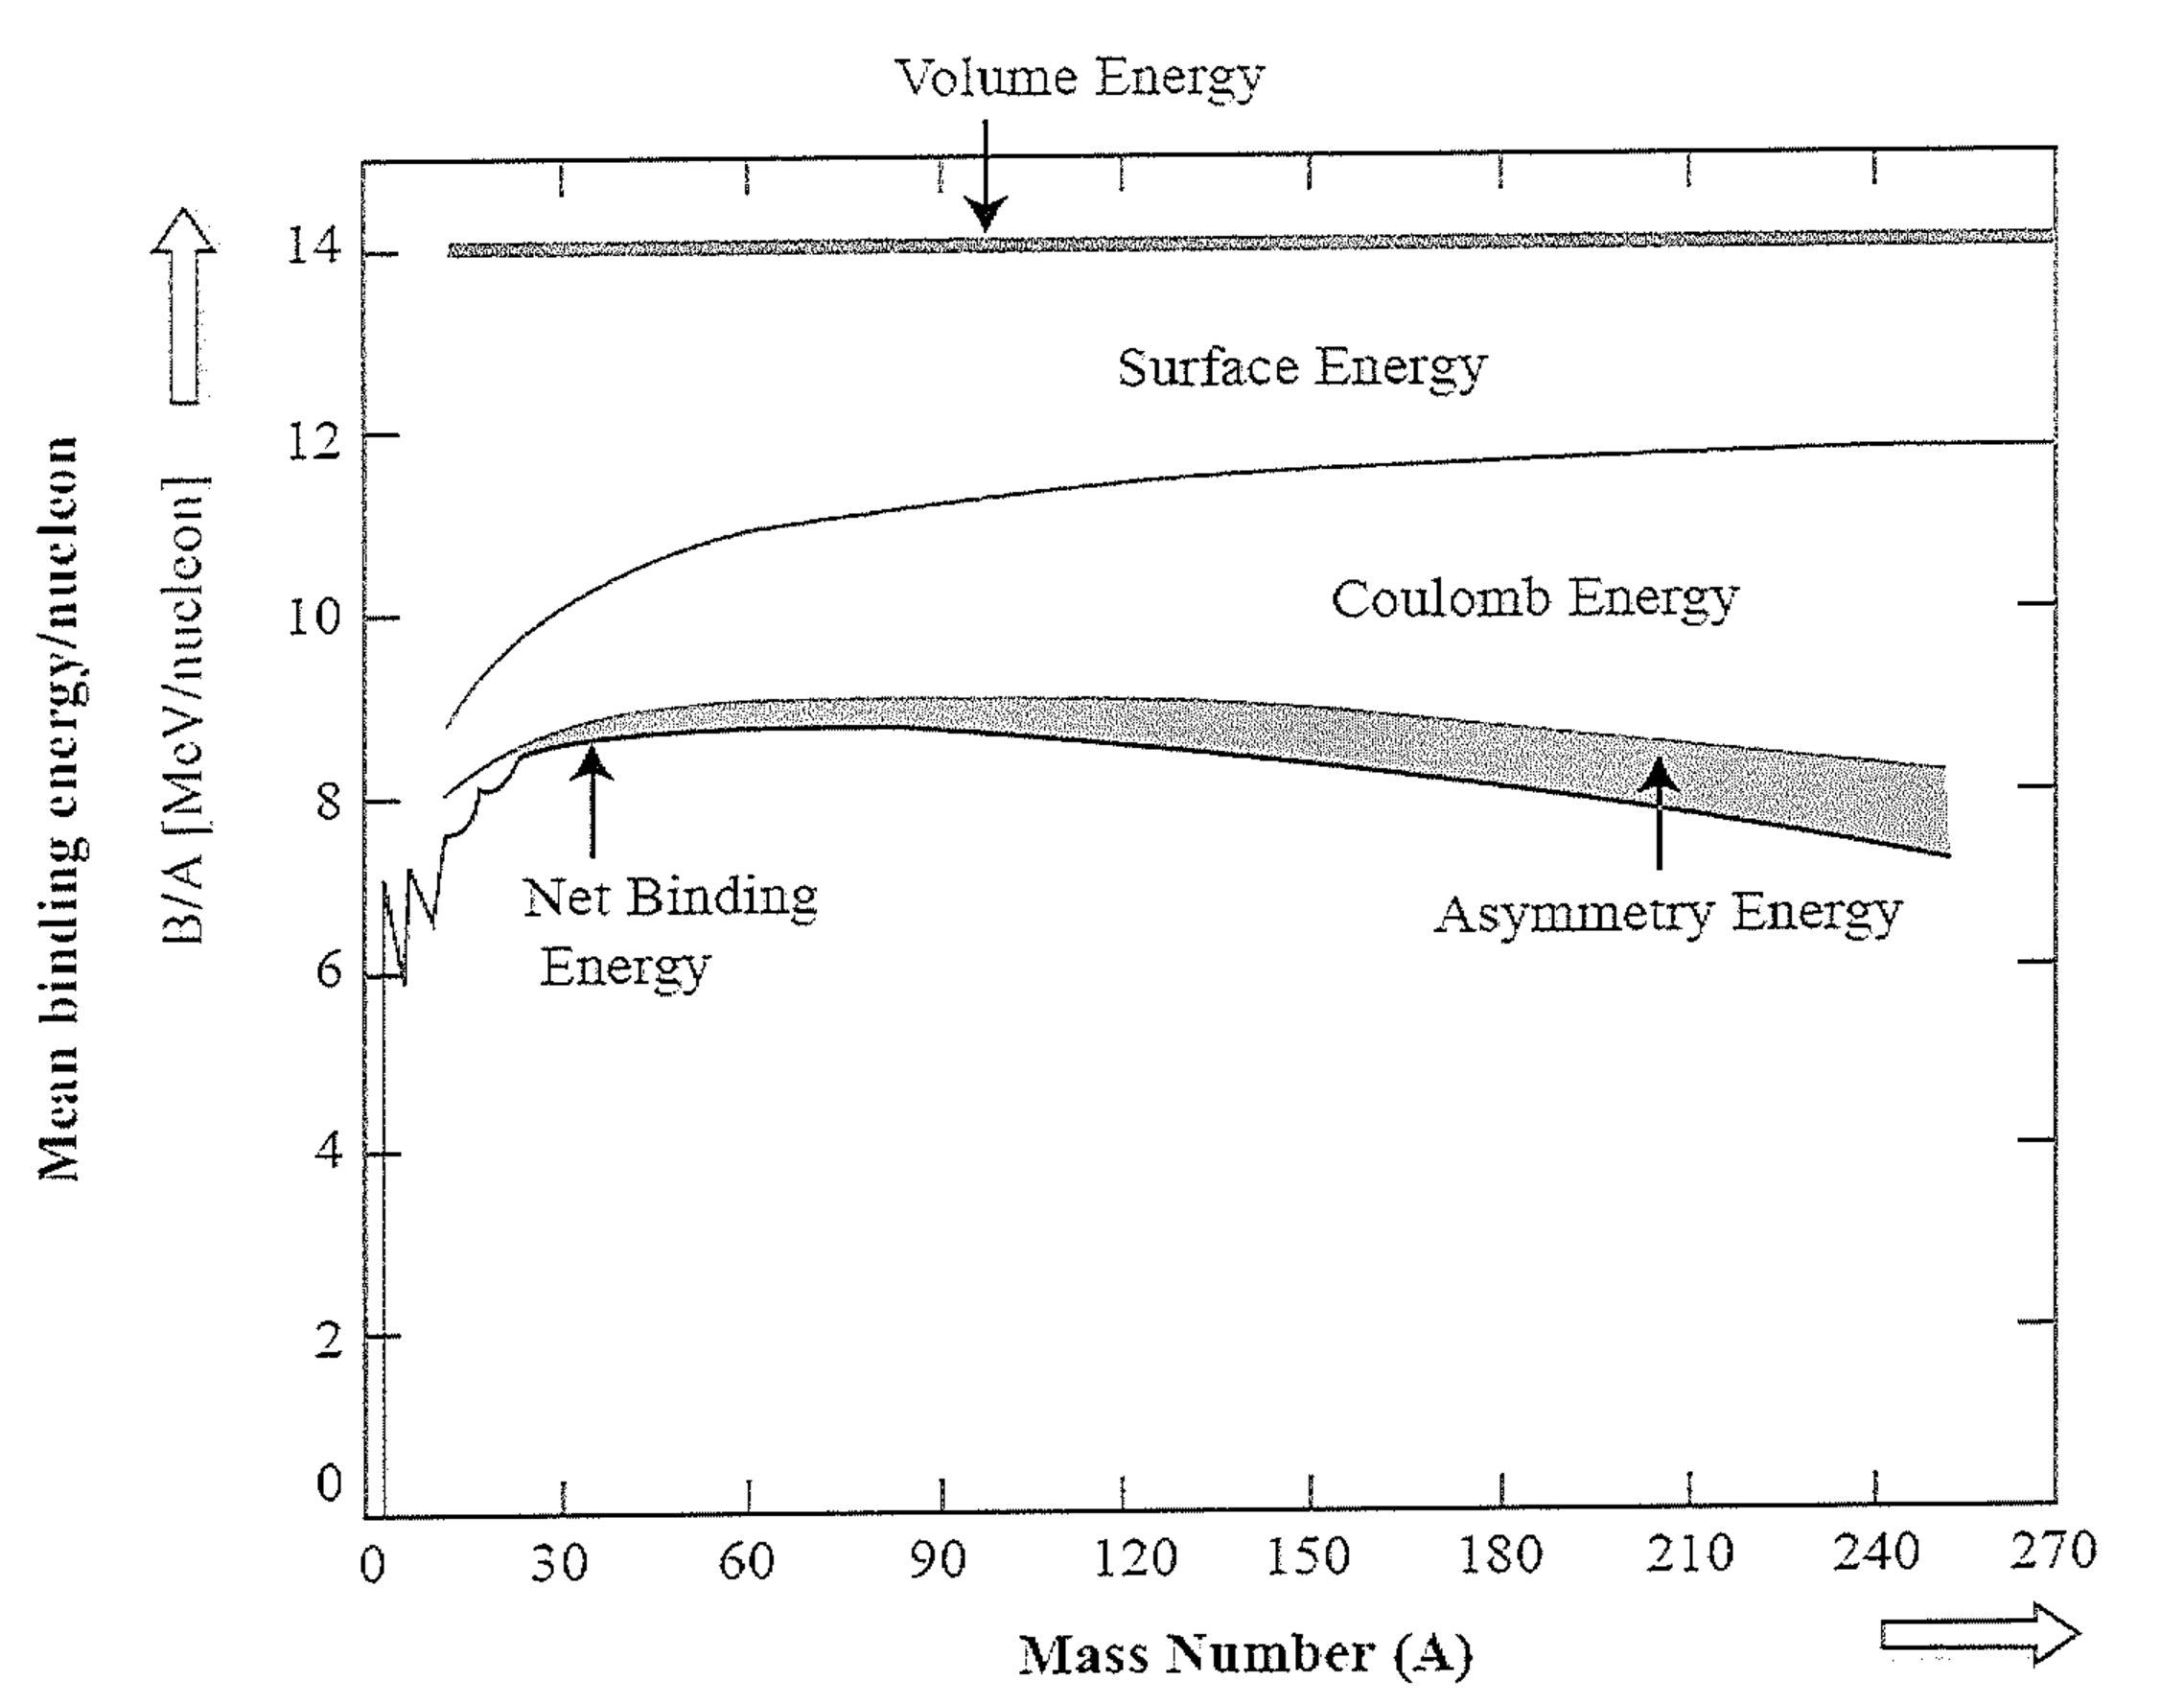
\includegraphics[width=4in]{images/rd/binding-effect.png}
        \caption{Relative Contributions to the Binding Energy Per Nucleon Showing the Importance of the Various Terms in te Semi-empirical Weizacker Formula \label{binding-effect}}
    \end{figure}
\end{enumerate}

\end{enumerate}


\end{document}
